% ==> START: Preamble
\documentclass[twoside]{extarticle}                                    % Extended article class (twoside for fancyhdr functionality)

% -- Required packages
\usepackage{amsmath, amsthm, sfmath, enumitem, graphicx, color}        % Standard packages
\usepackage[utf8]{inputenc}                                            % To generate table of contents
\usepackage[margin = 1in]{geometry}                                    % Set margins 1 inch on all sides
\usepackage{hyperref}                                                  % URL linking
\usepackage{lastpage}                                                  % Keep track of the page count
\usepackage{fancyhdr}                                                  % Better control over header and footer

% -- Document preferences
\raggedbottom{}                                                        % No extra space between paragraphs
\renewcommand{\familydefault}{\sfdefault}                              % Sans-serif font, sans-serif math (requires sfmath)
\numberwithin{equation}{section}                                       % Number equations within each section: <Sec#>.<Eqn#>
\setcounter{section}{-1}                                               % To start section numbering at zero

% -- Header and footer styling
\pagestyle{fancy}                                                      % Set the page style to default
\fancyhf{}                                                             % Clear the default fancy header and footer
\fancyhead[LE,RO]{CAAM 37830: Team 8}                                  % Authors (in brief)
\fancyhead[RE,LO]{\leftmark}                                           % Current section
\fancyfoot[LE,RO]{\url{https://github.com/caam37830/project-group-8}}  % Link to our GitHub repo
\fancyfoot[RE,LO]{Page \thepage{} of \pageref{LastPage}}               % Print page count (of total pages)
\renewcommand{\headrulewidth}{0.5pt}                                   % Set headrulewidth to 0.5pt (the line between content and header)
\renewcommand{\footrulewidth}{0.5pt}                                   % Set footrulewidth to 0.5pt (the line between content and footer)

% -- Document metadata
\title{Simulating Disease Spread with the SIR Model and Python}        % Document title
\author{Jarrod Dominguez, Anna Schouten, and Jack Potrykus}            % Document authors
\date{\today}                                                          % Document last-modified date
% <== END: Preamble

% -- Document content starts here
\begin{document}

% -- Title page
\maketitle{}           % Make title page
\thispagestyle{empty}  % Remove fancyhdr styling for the bibliography
\tableofcontents{}     % Show table of contents
\vfill{                % Note to reader/grader regarding length of this paper
    \begin{center}
        {\small\emph{Please note that the report itself spans pages 2 to 11 (10 total pages)}}
    \end{center}
}


% -- Main document
\newpage{}                                                             % New page, so it is clear that the report itself is <= 10 pages in length
\section{Abstract}
The SIR model is a method for modeling the spread of disease in a population based on the idea that the individuals in the population fall in to one of three categories: susceptible, removed, or infected.
\textbf{Susceptible} individuals have not yet gotten the disease and are in danger of contracting it.
\textbf{Infected} individuals are carriers of the disease and spread it to others.
\textbf{Removed} (alternatively, \textbf{recovered}) individuals have either recovered from the disease or died, so are no longer susceptible to it. We have implemented the SIR model using both an Agent-based model and a system of ODEs.
In our simulations and their extensions, we observe (under simple model parameters and constraints) effects of reinfection, social distancing, herd immunity, and more COVID-19 buzzwords, providing some simulated motivation for further real-life data-driven research into these topic.
Finally, all of this is accomplished via our Python library, \texttt{sir}, which offers multiple methods -- both discrete and continuous, scientific and just for fun -- of simulating disease spread using this canonical model.


\section{Introduction to SIR Model and Python Implementation}
We explore the SIR model both with a spatial component and without. For the spatial case, both methods use parameters \texttt{p}, \texttt{q} and \texttt{k} to represent how the disease spreads. The parameter \texttt{p} represents the maximum distance that an agent can move per period, \texttt{q} represents the radius around an infected individual that the disease can spread, and \texttt{k} represents the fraction of the infected population that recovers each day.

In the traditional SIR model with no spatial component, \texttt{p} and \texttt{q} are replaced with one variable \texttt{b}, which represents the number of infected agents per infected agent per period. In our discussion of these models we have used the following notation:
\begin{itemize}[itemsep = 0em]
    \item \texttt{i}: fraction of the population that is infected, with initial conditions \texttt{i0}. The aggregate number is denoted \texttt{I}, with initial conditions \texttt{I0}.
    \item \texttt{r}: fraction of the population that is removed, with initial conditions \texttt{r0}. The aggregate number is denoted \texttt{R}, with initial conditions \texttt{R0}.
    \item \texttt{s}: fraction of the population that is susceptible, with initial conditions \texttt{s0}. The aggregate number is denoted \texttt{S}, with initial conditions \texttt{S0}.
    \item \texttt{N}: number of individuals in the population (constant).
    \item \texttt{t}: time
\end{itemize}
The agent-based model uses interactions between infected individuals and susceptible individuals to trace the spread of the disease; the ODE method uses time dependent variables for each of the three possible states to model the spread of the disease. The evolution of these variables is described by the system of equations:
\begin{align}
    \frac{dr}{dt} &= k \cdot i(t) \\
    \frac{di}{dt} &= b \cdot s(t) \cdot i(t) - k \cdot i(t) \\
    \frac{ds}{dt} &= -b \cdot s(t) \cdot i(t)
\end{align}
We also explore three extensions to the above models, two of them being related to the agent based model and the other being related to the ODE model. We provide a brief introduction to each below.


\subsection{Structure of the \texttt{sir} Python Package}
The \texttt{sir} package contains five submodules:
\begin{enumerate}[label = (\roman*), itemsep = 0em]
    \item \href{https://github.com/caam37830/project-group-8/blob/main/sir/agent.py}{\texttt{agent}}, which contains class definitions for \texttt{Agent} and \texttt{DiscreteAgentModel}, which are necessary to carry out the discrete agent simulations with no spatial component.
    \item \href{https://github.com/caam37830/project-group-8/blob/main/sir/ode.py}{\texttt{ode}}, which contains class definitions for \texttt{OdeSir} and \texttt{SpatialSirOde}, which are necessary to carry out the ODE version of the problem (without/with spatial component, respectively).
    \item \href{https://github.com/caam37830/project-group-8/blob/main/sir/smartagent.py}{\texttt{smartagent}}, which contains class definitions for \texttt{SmartAgent} and \texttt{SmartAgentModel2D}, which are necessary to carry out the discrete agent simulations with spatial component, and can be used to model “intelligent” agent behavior along with the standard random behavior, for use in the \textbf{smart agent extension}.
    \item \href{https://github.com/caam37830/project-group-8/blob/main/sir/reinfect_ode.py}{\texttt{reinfect\_ode}}, which contains the class definition for \texttt{ODEReinfection}, which inherits from \texttt{OdeSir}; this is used in the \textbf{reinfection extension}.
    \item \href{https://github.com/caam37830/project-group-8/blob/main/sir/conway_agent.py}{\texttt{conway\_agent}}, which contains class definitions for \texttt{ConwayAgent} and \texttt{ConwayModel}, which are necessary for the \textbf{Conway extension}.
\end{enumerate}
In addition you will find the directories \href{https://github.com/caam37830/project-group-8/tree/main/test}{\texttt{test}}, containing unit tests of functionality for each implementation, \href{https://github.com/caam37830/project-group-8/tree/main/Scripts}{\texttt{Scripts}}, which contains scripts to be run on the Midway Compute Cluster, and \href{https://github.com/caam37830/project-group-8/tree/main/doc}{\texttt{doc}}, which contains our \href{https://github.com/caam37830/project-group-8/tree/main/doc/final/plots}{plots} and \href{https://github.com/caam37830/project-group-8/tree/main/doc/final/conway_plots}{animations}, the \href{https://github.com/caam37830/project-group-8/blob/main/doc/checkpoint/checkpoint.md}{midway checkpoint}, and the document you're reading! System requirements to use the package can be found in \href{https://github.com/caam37830/project-group-8/blob/main/requirements.txt}{\texttt{requirements.txt}}, and more useful info about this repository can be found in \href{https://github.com/caam37830/project-group-8/blob/main/README.md}{\texttt{README.md}}.


\subsection{Jarrod Dominguez: Overview of the Smart Agent Extension}
We explore how the spread of the virus is effected if the agents take some effort to socially distance themselves from others, if given enough information about the disease. We define the following parameters that are specific to this extension:
\begin{itemize}[itemsep = 0em]
    \item \texttt{knowledge\_distance (kd)}: the radius around an individual from which they can gather knowledge
    \item \texttt{knowledge}: the cumulative sum of infected and recovered individuals within the \texttt{knowledge\_distance} of an individual
    \item \texttt{knowledge\_threshold (kt)}: the knowledge score that an infected agent must have to socially distance itself from healthy agents
    \item \texttt{fear\_distance (fd)}: the radius around an individual from which they can gather become more fearful of the disease
    \item \texttt{fear}: the cumulative sum of infected individuals within the \texttt{fear\_distance} of an individual
    \item \texttt{fear\_threshold (ft)}: the fear score that a healthy agent must have to socially distance themselves from infected agents
\end{itemize}
Once a healthy agent achieves a fear score above the threshold level, they will then chose the location within a distance \texttt{p} that maximizes the sum of distances between them and any infected agents that are within the \texttt{fear\_distance} from them. Furthermore, once an infected agent achieves a knowledge score above the threshold level, they will maximizes the sum of distances between them and healthy individuals within the \texttt{knowledge\_distance} from them. Recovered individuals, and individuals that have not surpassed threshold levels do not act in any intelligent manner so they just chose a random location, within radius \texttt{p}, to move to each period.


\subsection{Anna Schouten: Overview of the Reinfection Extension}
Our previous models are dependent on the assumption that individuals can only be infected by the virus once. We investigate the model adjusted to account for reinfection rate. In order to account for reinfection, we also accounted for death rate due to the virus, such that infected individuals either recovered or died, rather than assuming that all previously infected individuals belonged to a single category. These changes resulted in a new system of differential equations described in detail below. Rather than a S, I, R model, the system represents a S, I, R, \textbf{D} model, where $d(t)$ corresponds to the proportion of the population that dies due to the virus over time. Additionally, new parameters \texttt{e} and \texttt{g} are added to the new model. The parameter \texttt{g} represents probability of reinfection, and the parameter \texttt{e} represents the death rate. We monitor how the probability of reinfection changes the evolution of the groups within the population over time.


\subsection{Jack Potrykus: Overview of the Conway Extension}
The homework exercise on Conway's ``Game of Life'' was fascinating to me, not only for the fun of implementing sparse matrix arithmetic, but also because I learned more about the history of Conway's Game of Life. While the grader of this paper likely knows the history, my parents did not, so a brief synopsis of what I found interesting: Conway's Game of Life is deterministic, and \emph{Turing complete}! Deterministic meaning that the state of which cells are ``alive'' at time period $t$ can be uniquely determined via its starting position, and Turing complete (broadly) meaning that it is a system in which we can ``write'' a program/computation and receive an ``answer'' as output (this requires some mental gymnastics, as animated pentominos on a grid of arbitrary size is not our usual method of calculation). My extension implements the SIR model \emph{on top} of Conway's Game of Life, producing a new zero-player game with two ``turns'' per time-step: first, Conway's turn; next, the disease's turn.


\section{The Basic SIR Model}
We investigate a variety of different simulations but will discuss only the most interesting in this section (for more on this model and a discussion of other simulations see the midterm checkpoint). The choice of \texttt{b} and \texttt{k} is of great importance in how both of these methods model the spread of disease through a population. The higher \texttt{k} is the faster any given individual will recover from the disease, and thus the less time they will be able to infect people. On the other hand, a high \texttt{b} will lead to many agents being infected each period. Ultimately, increasing the initial number infected or \texttt{b} generally will lead to more people getting infected faster and the disease being more successful overall, while increasing \texttt{k} will have the opposite effect.

Generally, the ODE model and the agent based model provide similar dynamics to how the virus will progress through a population. We chose to highlight a simulation in which the two approaches do not agree (discrete agent results on the left, ODE results on the right):
\begin{center}
    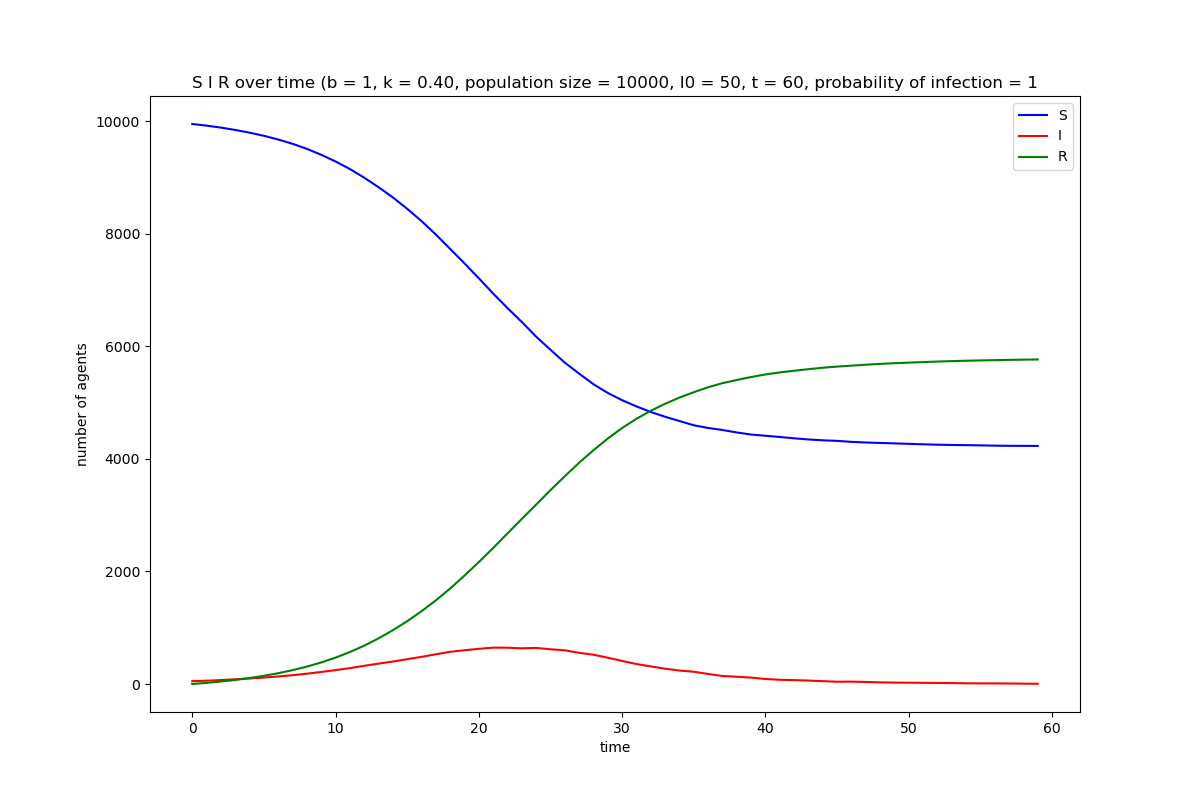
\includegraphics[trim = {3cm 1cm 3cm 1cm}, clip, width = 0.45\linewidth]{../../checkpoint/plots/k40Agent.png} \qquad
    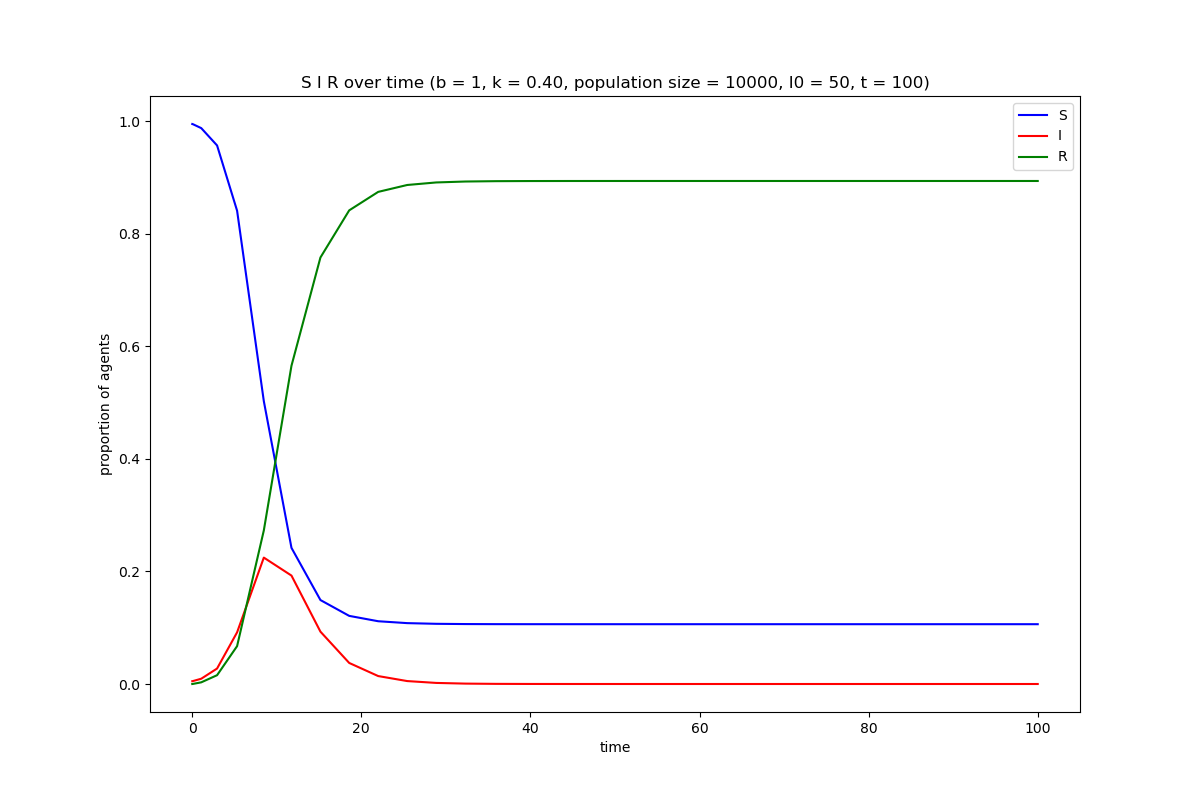
\includegraphics[trim = {3cm 1cm 3cm 1cm}, clip, width = 0.45\linewidth]{../../checkpoint/plots/k40ODE.png}
\end{center}
These two models have the same parameters, yet the ODE model seems to create drastically different results than the agent based approach. This seems odd at first, but a small nudge in the direction of increased infections can lead to a much worse outcome overall. For example, consider that the infection rate is the same as the recovery rate if there are 50 agents that are infected. Then, we could expect the number of agents who are sick to not increase that much. However, if we nudge that number up a little bit, say to 70, then we have pushed the system out of equilibrium and the infections may get out of control, this is the idea of flattening the curve and trying to keep the number of infections manageable. This example is important to keep in mind for not only the spatial model, but the extensions as well as it indicates how important our model assumptions are to the dynamics of a disease.


\section{Spatial Component Implementation}
\subsection{Discrete Agent Model}
For the discrete agent spatial model we first need to understand how our choice of parameters effects the timeline of the virus. Unlike in the non-spatial model, the population size plays a huge role in the dynamics of the virus since we fix the world to a $1 \times 1$ square. Thus, the higher the population the more densely packed our agents are and this leads to the virus spreading more quickly even with a low value of \texttt{q}. Both \texttt{p} and \texttt{q} have positive relationships with the rate of spread, which makes sense. If individuals have a large radius of infection, then they infect more people per period, and if they move a large distance, then the chance that an infected person interacts with agents that they haven't interacted with before also increases. This leads to our first simulation in which we start with 5 infected agents near the center of the population and see how the virus spreads holding all constant between simulations but the distance that agents can move per period \texttt{p}.
\begin{center}
    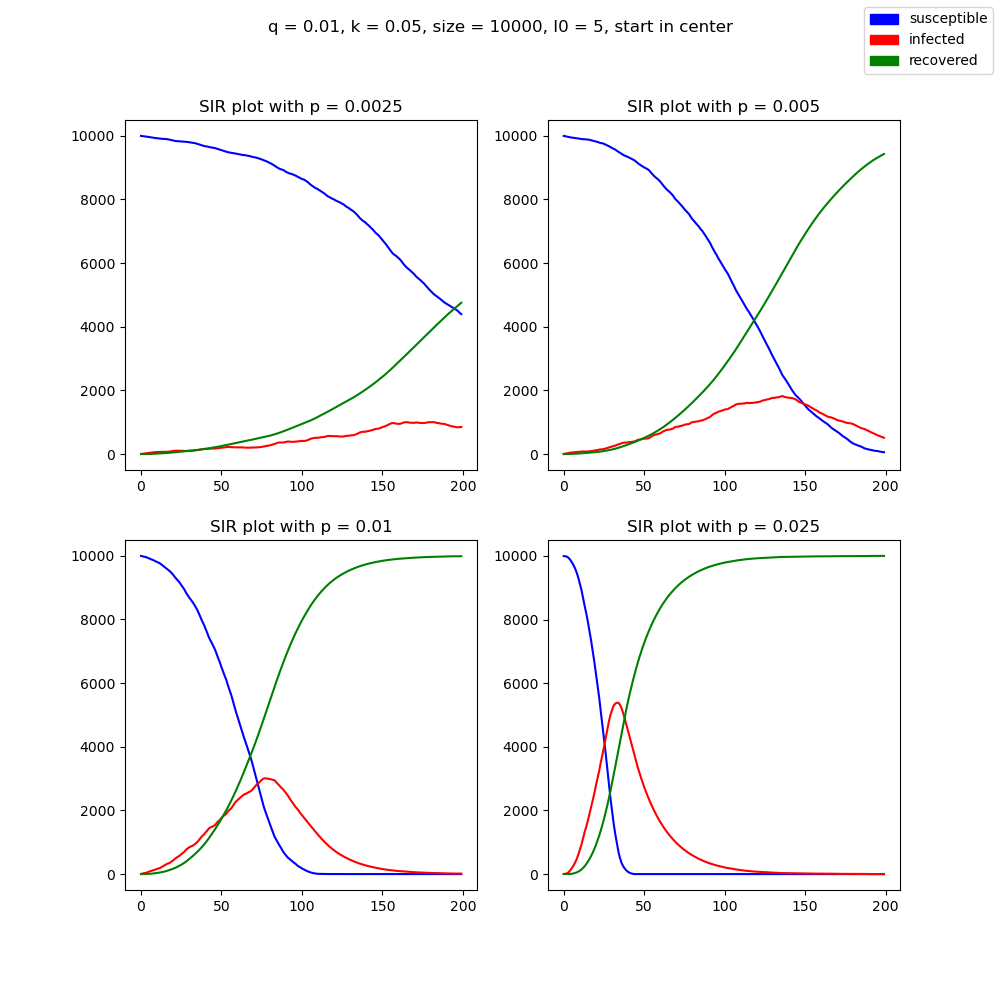
\includegraphics[trim = {1.5cm 2cm 0cm 0}, clip, width = 0.55\linewidth]{../plots/startmid.png}
\end{center}
We observe that the further an agent can move per period the faster the disease spreads, as hypothesized. We also see that a $\texttt{p} \in (0.005,0.01)$ will produce a progression of the disease that infects almost all agents over the course of the 200 day range that we use. Next, we are interested in how the starting location of infected agents effects the overall spread of the disease. We chose and \texttt{p = 0.0075} and keep all other parameters the same as the first simulation and now vary the starting location of the infected agents:
\begin{center}
    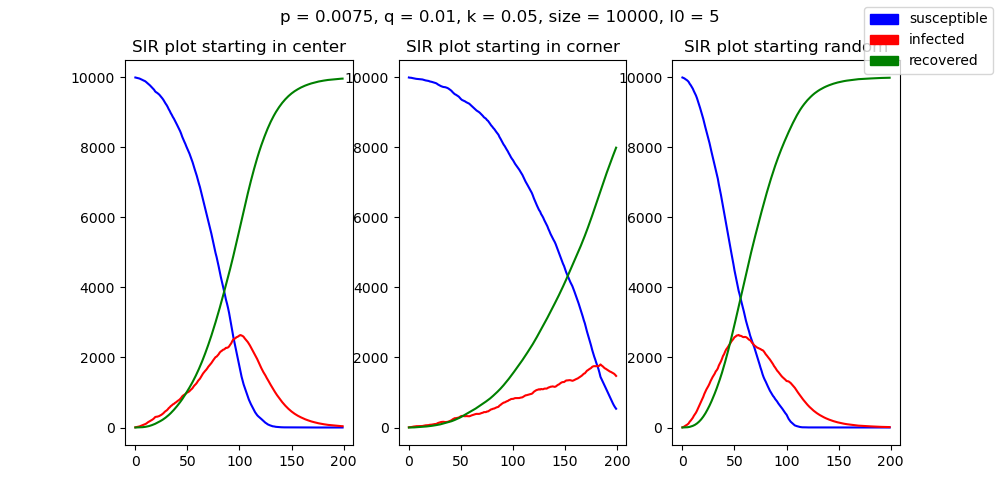
\includegraphics[trim = {1.5cm 0 0 0}, clip, width = 0.65\linewidth]{../plots/startdiff.png}
\end{center}
We observe that the virus is the most successful when the agents are randomly placed, which seems counterintuitive at first. However, since we have chosen parameters that lead to the disease spreading throughout the entire population it will be advantageous for the disease to have as few overlapping infected in the early stages as possible, which leads the the random placement being more effective at spreading the disease than the grouping in the center. The simulation in which that agents are placed in the corner provides the slowest spread of the disease which makes sense as it not only suffers from the grouping issue that we see when the agents are in the center, but the disease can only spread in 2 directions.


\subsection{Differential Equations Model}
For the differential equation model, to account for spatial components, the ODEs become PDEs. The differential model is simulated on a $M \times M$ grid, and the PDE model has a diffusion term that is multiplied by a parameter \texttt{p}, analogous to parameter \texttt{p} in the agent-based model. However, to account for step size in the differential model, \texttt{p} as compared to the agent-based parameter is scaled by 1/M. As with the spatially-independent models, we see that the dynamics of the agent-based model and the differential equation are similar. However, the change in values of \texttt{p} does not have the same impact on results. With parameters \texttt{N = 10000, b = 1, k = 0.05, i0 = 0.1}, and a $200 \times 200$ grid, the results over various values of \texttt{p} appear below.
\begin{center}
    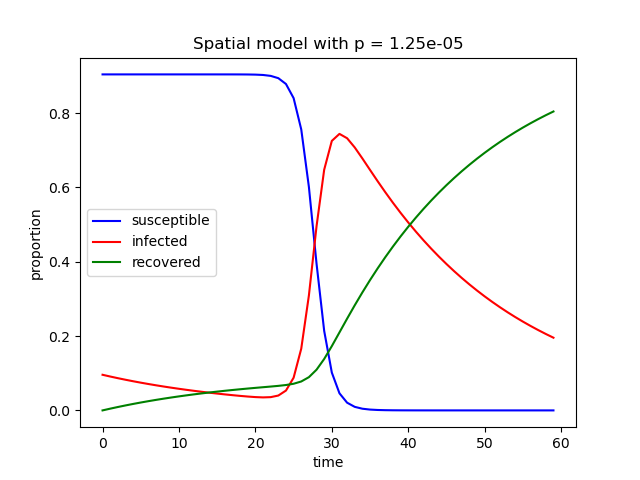
\includegraphics[trim = {0.5cm 0 0.5cm 0.5cm}, clip, width = 0.40\linewidth]{{../plots/spatialp_1.25e-05}.png} \qquad
    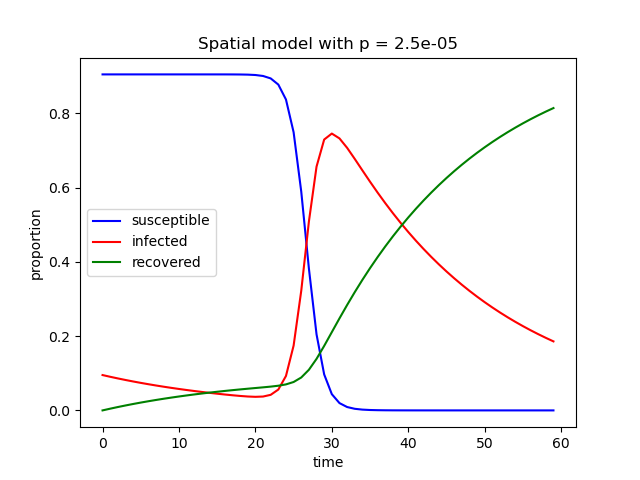
\includegraphics[trim = {0.5cm 0 0.5cm 0.5cm}, clip, width = 0.40\linewidth]{{../plots/spatialp_2.5e-05}.png} \\
    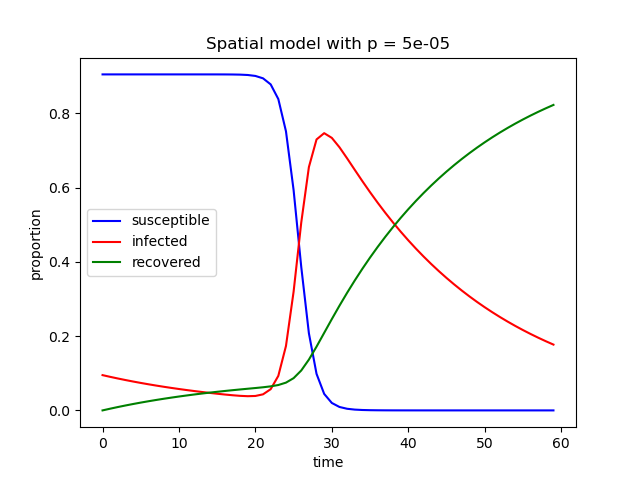
\includegraphics[trim = {0.5cm 0 0.5cm 0.5cm}, clip, width = 0.40\linewidth]{{../plots/spatialp_5e-05}.png} \qquad
    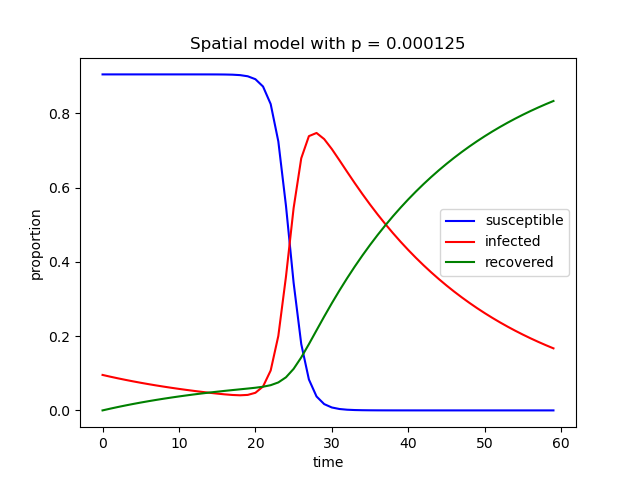
\includegraphics[trim = {0.5cm 0 0.5cm 0.5cm}, clip, width = 0.40\linewidth]{{../plots/spatialp_0.000125}.png}
\end{center}
The change in parameter \texttt{p} seems to have little to no influence on the development of the model.  Similarly, the location of the initial infected population is less significant. For the same parameters as above and \texttt{p = 0.000075}, we show plots of the initial population in the center, corner, and at random (top left, top right, and bottom, respectively) below. All three locations seem to produce essentially the same results; overall, this model seems to be largely unaffected by the spatial components, with results that seem to be relatively spatially-independent.
\begin{center}
    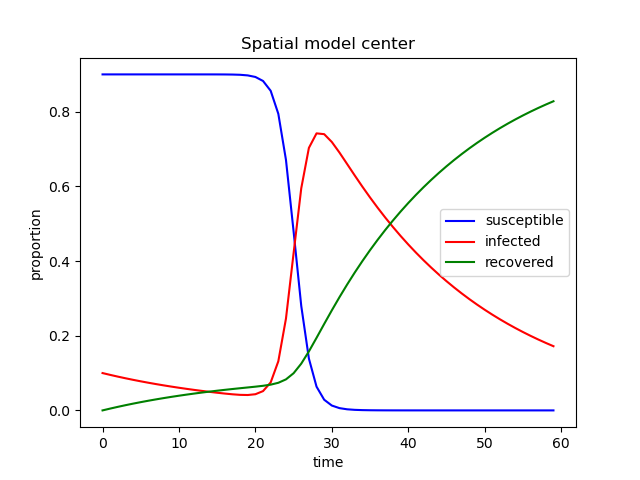
\includegraphics[trim = {0.5cm 0 0.5cm 0.5cm}, clip, width = 0.40\linewidth]{../plots/spatial_center.png} \qquad
    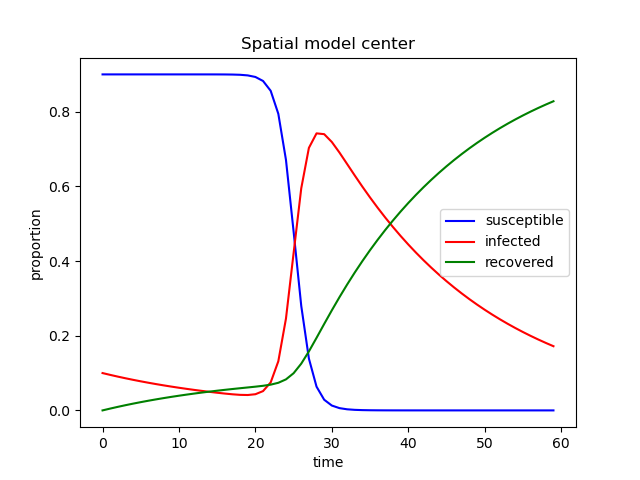
\includegraphics[trim = {0.5cm 0 0.5cm 0.5cm}, clip, width = 0.40\linewidth]{../plots/spatial_corner.png} \\
    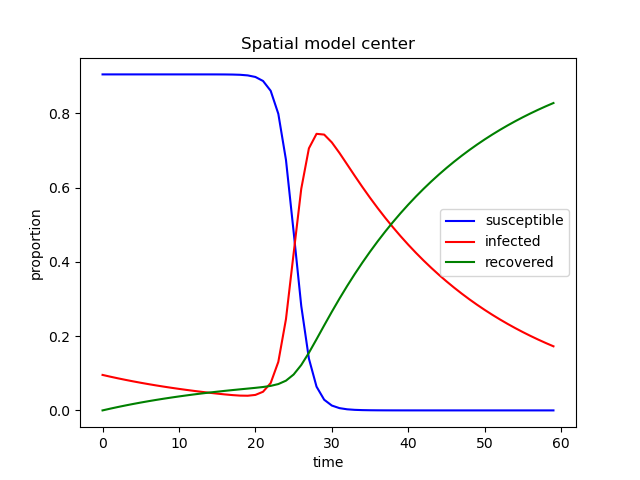
\includegraphics[trim = {0.5cm 0 0.5cm 0.5cm}, clip, width = 0.40\linewidth]{../plots/spatial_random.png}
\end{center}


\section{Extensions of the SIR Model}
\subsection{Jarrod Dominguez: Smart Agent Extension}
Throughout history, we have faced various diseases and have found that social distancing and quarantines have been one of the best ways to combat the spread (Roos (2020)). So, we propose the question: How does the course of a disease spreading change if the agents make intelligent decisions to slow its spread?

The figure below and on the left depicts a baseline simulation where agents do not do anything to slow the spread.
The figure below and on the right has the same parameters, except this time the agents have a \texttt{fear\_threshold} and \texttt{knowledge\_threshold} of $1000$, and a \texttt{fear\_distance} and \texttt{knowledge\_distance} of $0.1$.
\begin{center}
    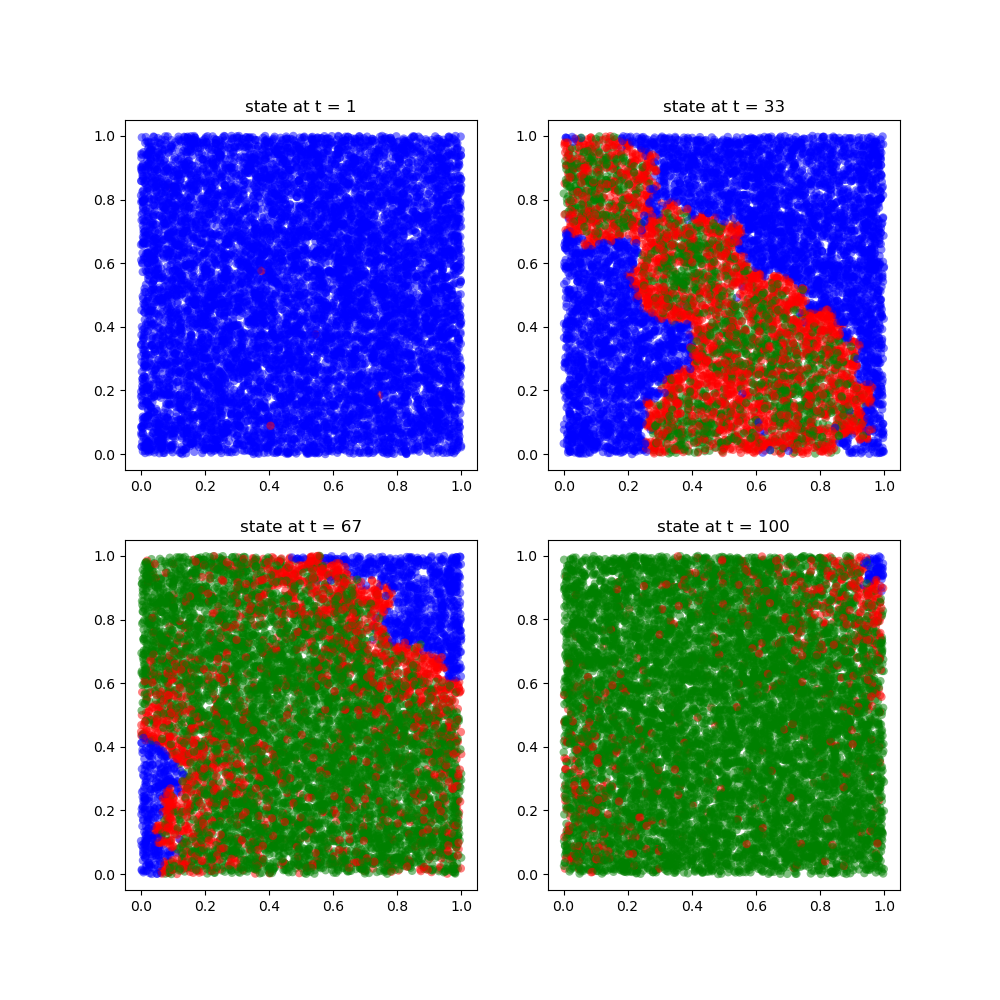
\includegraphics[trim = {2.4cm 2cm 0 0}, clip, width = 0.45\linewidth]{../plots/nolearn.png} \qquad
    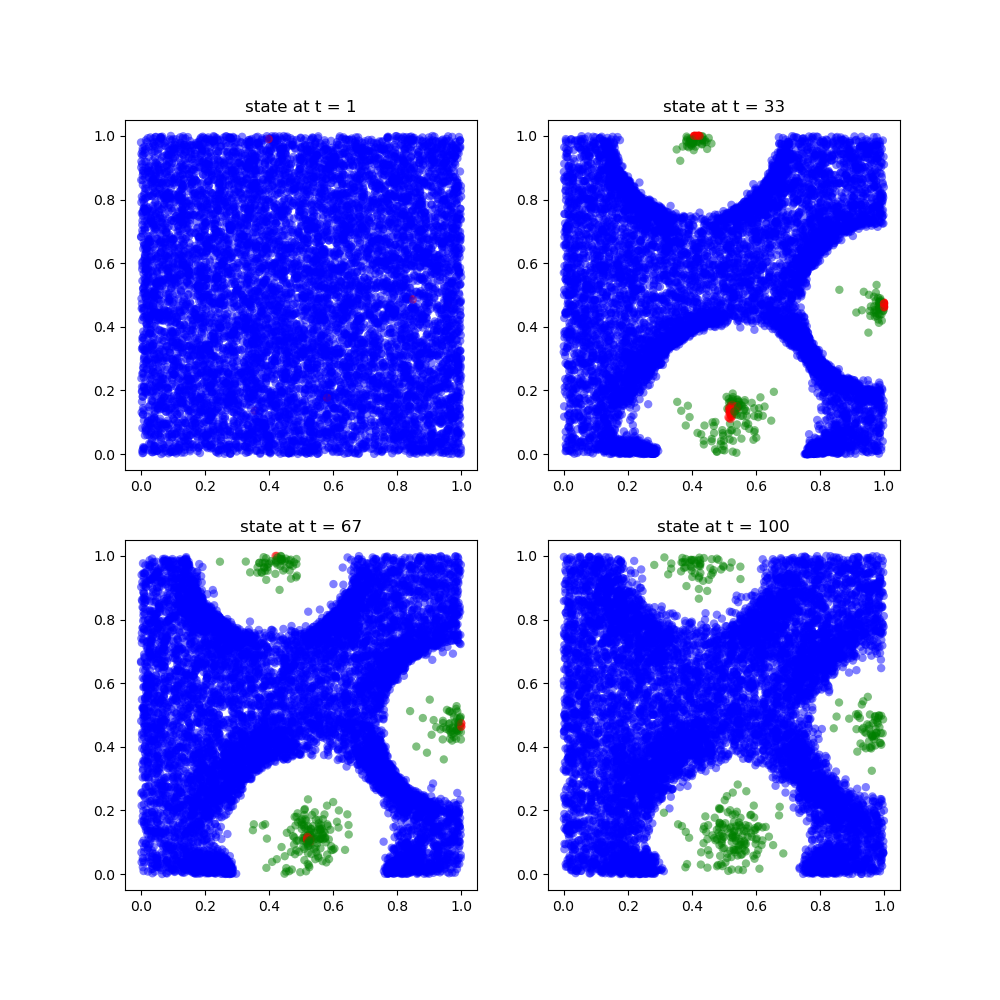
\includegraphics[trim = {2.4cm 2cm 0 0}, clip, width = 0.45\linewidth]{../plots/yeslearn.png}
\end{center}
In the ``baseline'' agent simulation with these parameters, the virus runs rampant through the population. After 67 days most of the population has already been infected and by 134 days everyone has been infected with the disease and most agents have recovered. We chose to show a simulation with parameters that lead to widespread contraction of the virus to emphasize how important social distancing could be.

In the ``smart'' agent simulation, observe that on day 67 the scattershot tells an entirely different story. We see that groups of healthy individuals have isolated themselves from the sick and vice-versa. The most interesting plot, however, is of day 134 in which we see that the areas that fair best against the virus are actually those that have had the opportunity to learn about the virus and distance themselves. We see a large cluster of healthy individuals in the center of the plot because they had the opportunity to learn about the disease before it got out of control in their region whereas the top left corner did not protect itself against the disease because its agents were not able to learn about the disease before a critical number of infected agents were present. Finally, on day 200, we see the residual effects of social distancing where their is still some separation between recovered individuals and susceptible ones, but it is much diminished from when the virus was at its peak.

Of course these simulations are stylized in a manner to prove a point about the importance of taking advantage of every tool possible to thwart the spread of disease, so the real world implications are limited. For example, we would like to include some strategic behavior beyond the agents just moving to a specific point with certainty, meaning that agents would make assumptions about how other agents would move and would use that information as well to help make their decisions (Kamien \& Schwartz (2012)). All agents also may not ``behave'', they may refuse to learn or actually act destructively, which would blur the quarantine radii that we observe on day 67 of the ``smart'' simulation. Modeling human behavior, however, is a tall task and proving the merits of social distancing in a constrained case can lead us down the correct path in future research.


\subsection{Anna Schouten: Reinfection Extension}
For some diseases, an individual previously infected cannot become reinfected because the immune system recognizes the disease and produces antibodies. However, in the case of many diseases, including COVID–19 (Murillo-Zamora, 2020), there is some probability of reinfection. The question we have considered is how the probability of reinfection influences in the overall rate of infection and recovery. To accurately reflect these conditions, the new model also accounts for the rate of deaths due to the disease. This is described by the following system of differential equations:
\begin{align}
    \frac{ds(t)}{dt} &= -b \cdot s(t) \cdot i(t) + g \cdot r(t) \\
    \frac{dr(t)}{dt} &= k \cdot i(t) - g \cdot r(t) \\
    \frac{di(t)}{dt} &= b \cdot s(t) \cdot i(t) - k \cdot i(t) - e \cdot i(t) \\
    \frac{dd}{dt}    &= e \cdot i(t)
\end{align}
In this system, as with the parent system, $b$ represents interactions and $k$ represents recover rate; $s$, $i$, and $r$ are unchanged. The new expression $dd / dt$ represents the death rate within the population, and $g$ is the rate of reinfection, with $e$ as the rate of death from the disease. Modeled with three different reinfection rates $g = 0.05, 0.1, 0.15$, with parameters $N = 10000, k = 0.25, b = 1$, and $e = 0.005$ fixed, appear below:
\begin{center}
    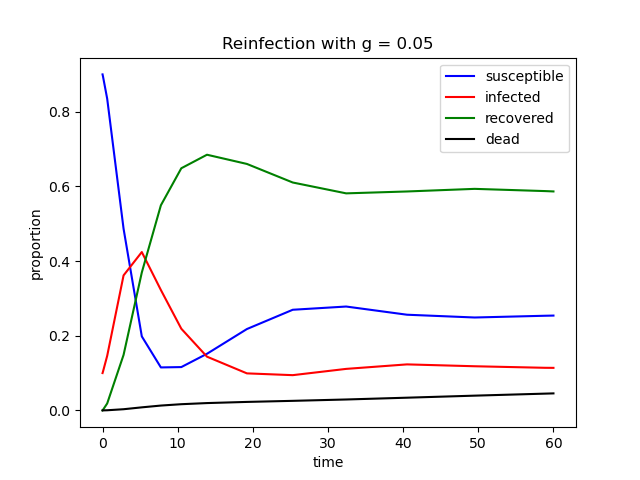
\includegraphics[width = 0.49\linewidth]{{../plots/reinfectg_0.05}.png}
    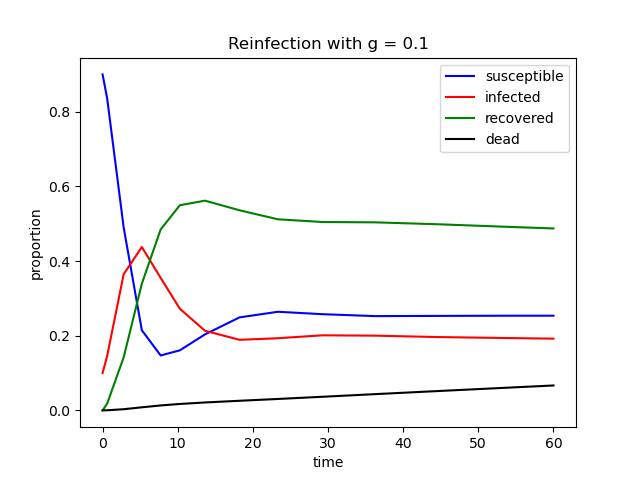
\includegraphics[width = 0.49\linewidth]{{../plots/reinfectg_0.1}.png} \\
    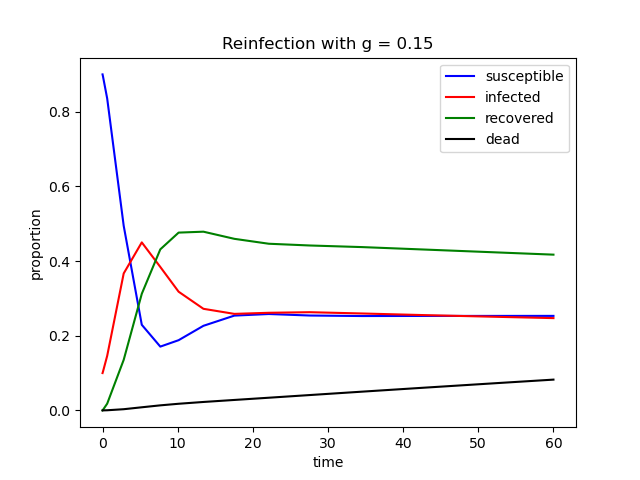
\includegraphics[width = 0.49\linewidth]{{../plots/reinfectg_0.15}.png}
\end{center}
In contrast to the previous model, the susceptible proportion of the population does not decrease and plateau. Instead, the decrease is followed by an increase before the proportion stabilizes. As the reinfection rate increases, the proportion of the population that is infected stabilizes at a value that is close to the stable susceptible proportion, and the proportion of the population that is recovered is much smaller. The proportion of the population that dies stays close to the same for all three reinfection rates but may be very slightly higher with the higher reinfection rate. Over time, it is possible that at higher reinfection rates, the proportion of infected individuals may be larger than the susceptible individuals.

The model could be changed slightly to model vaccinations. A vaccinated population would follow something similar to this model with a negative $g$ parameter. This difference would be that in the current model individuals moved from susceptible to infected before they can be recovered, but in the case of vaccinations, individuals would move directly from being susceptible to being recovered.


\subsection{Jack Potrykus: Conway Extension}
Conway's Game of Life's roots trace back John von Neumann's desire to model life itself as a reproducing Turing Machine (Wolfram, 2002). The game itself has been lauded as being particularly suited for simulating the growth of society: ``Because of Life's analogies with the rise, fall and alterations of a society of living organisms, it belongs to a growing class of what are called 'simulation games' (games that resemble real-life processes)."'' (Gardner, 1970). This prodigious background (and the compulsory nature of this assignment) make Conway's Game of Life both an appropriate and interesting extension of the classical SIR model.

Conway's Game of Life is considered to be a \emph{zero-player} game: after the initial input, it requires no additional input from the user, and can ``play'' indefinitely. This extension creates a new game: the Conway SIR model, which simulates SIR model on top of disease spread. The model parameters are changed slightly, although many are similar to the original discrete model:
\begin{itemize}[itemsep = 0em]
    \item \texttt{m} and \texttt{n} are the rows and columns, respectively, of the grid
    \item \texttt{k} is the proportion of infected who recover each day
    \item \texttt{p} is the probability of an agent being infected
\end{itemize}
So \texttt{p} is effectively a replacement for \texttt{b}, which in the discrete model is the number of interactions per day. Since the number of ``interacting'' agents is fixed (the cells neighboring that agent, including diagonals), we can adjust the probability of infection to change the rate of spread. Consider an agent which borders $\nu$ number of ``infected'' agents. Then their probability of being infected is $1 - (1 - p)^\nu$. The game is conducted as follows:
\begin{enumerate}[label = (\arabic*), itemsep = 0em]
    \item Receive parameters and initial state of each \texttt{ConwayAgent} from the user
    \item If the user requests the time period to advance (\texttt{step()}, \texttt{step\_t\_days()}, and \texttt{plot\_t\_days()} methods)
    \begin{enumerate}[label = (\roman*), itemsep = 0em]
        \item Advance the Conway grid and update which cells are alive
        \item Spread the disease, and recover some proportion of the sick agents
            \begin{itemize}[itemsep = 0em]
                \item Only infected agents who are ``alive'' in the Conway sense can infect susceptible agents
                \item Only agents who are ``alive'' in the Conway sense can be infected, or recover
                \item If an agent ``dies'' in the Conway sense, they keep their SIR state. For example, an infected, ``dead'' agent cannot infect anyone else, but also not recover. If that cell becomes ``alive'' later on, it will be in the ``infected'' state. This opens the possibility to ``second waves''.
            \end{itemize}
    \end{enumerate}
\end{enumerate}
Four simulations, each on a $50 \times 50$ board, are presented below\ldots but these are only the final frame of what are really animations! So click on each image to be taken to a ``live'' version of it, or visit \texttt{doc/final/conway\_plots/} in this repository to see them all (there are \emph{sixteen} animations on \emph{four} grid sizes there)! From left to right, top to bottom, the parameters changing are:
\begin{itemize}[itemsep = 0em]
    \item Probability of infection for each encounter with infected = 0.1, 0.3, 0.5, 0.7
    \item Proportion of cells \emph{initially} ``alive'' = 0.3, 0.4, 0.5, 0.6
    \item Proportion of cells \emph{initially} ``infected'' = 0.1, 0.2, 0.3, 0.4
\end{itemize}
Note that the last two changing parameters are \emph{not} model parameters; I wrote a separate function in \texttt{conway\_script.py} which will generate suitable test material, given these inputs. A legend for the color coding: {\color{blue} susceptible}, {\color{red} infected}, {\color{green} recovered}, with white squares being those which are ``dead'' in the Conway sense.
\begin{center}
    \href{https://github.com/caam37830/project-group-8/blob/main/doc/final/conway_plots/conway_m_50_n_50_k_0.1_p_0.1_pia_0.3_pii_0.1.gif}{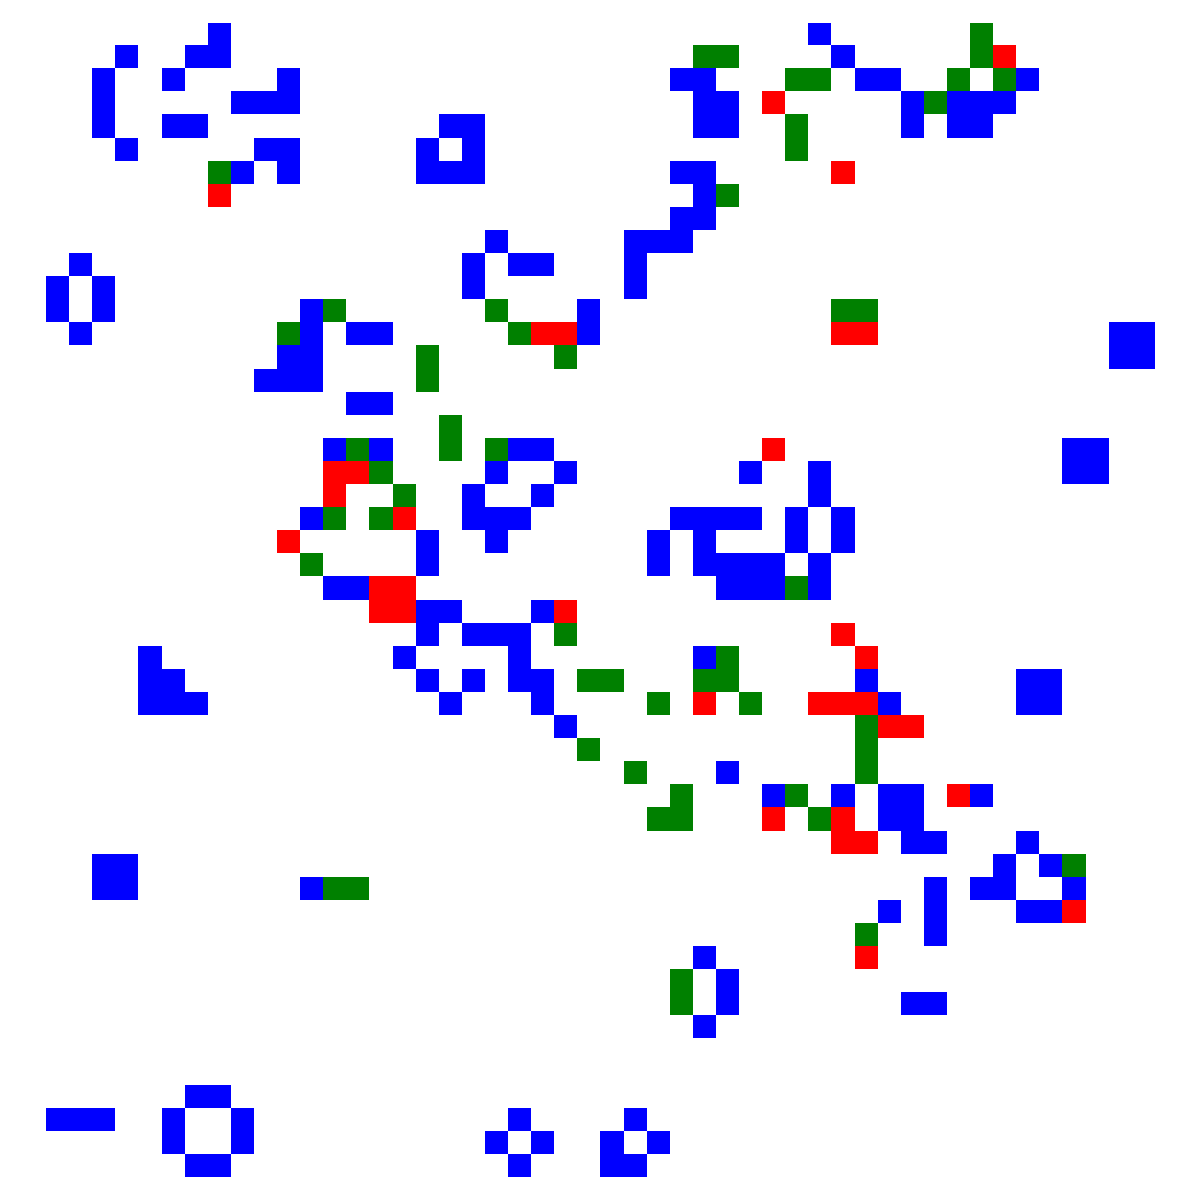
\includegraphics[width = 0.40\linewidth]{{../conway_plots/conway_static_p_0.1_pia_0.3_pii_0.1}.png}} \qquad
    \href{https://github.com/caam37830/project-group-8/blob/main/doc/final/conway_plots/conway_m_50_n_50_k_0.2_p_0.3_pia_0.4_pii_0.2.gif}{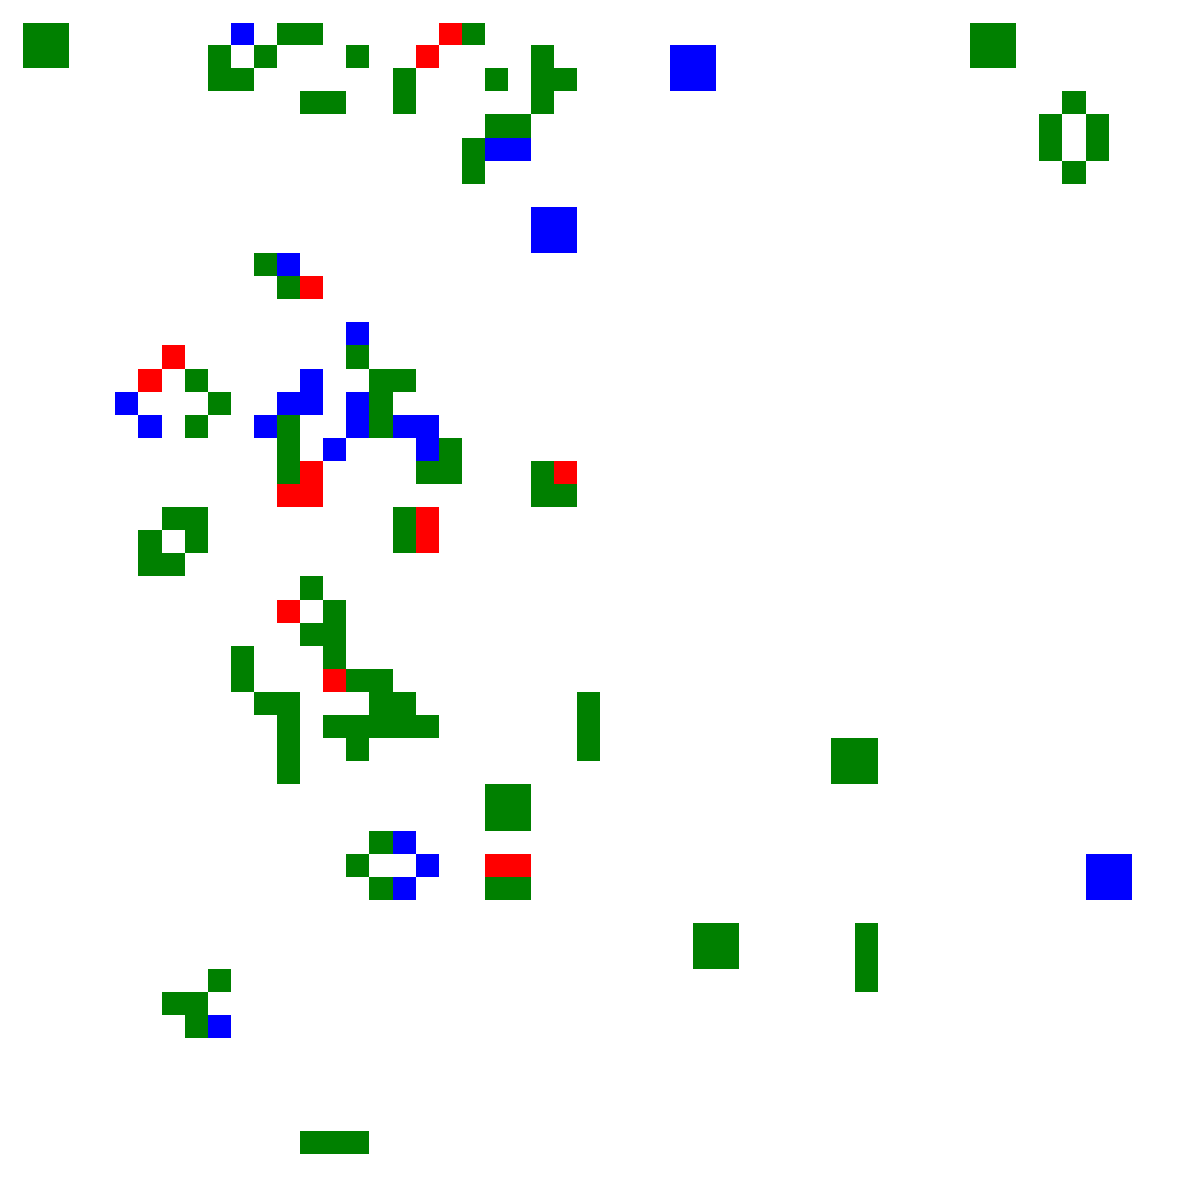
\includegraphics[width = 0.40\linewidth]{{../conway_plots/conway_static_p_0.3_pia_0.4_pii_0.2}.png}} \\
    \href{https://github.com/caam37830/project-group-8/blob/main/doc/final/conway_plots/conway_m_50_n_50_k_0.3_p_0.5_pia_0.5_pii_0.3.gif}{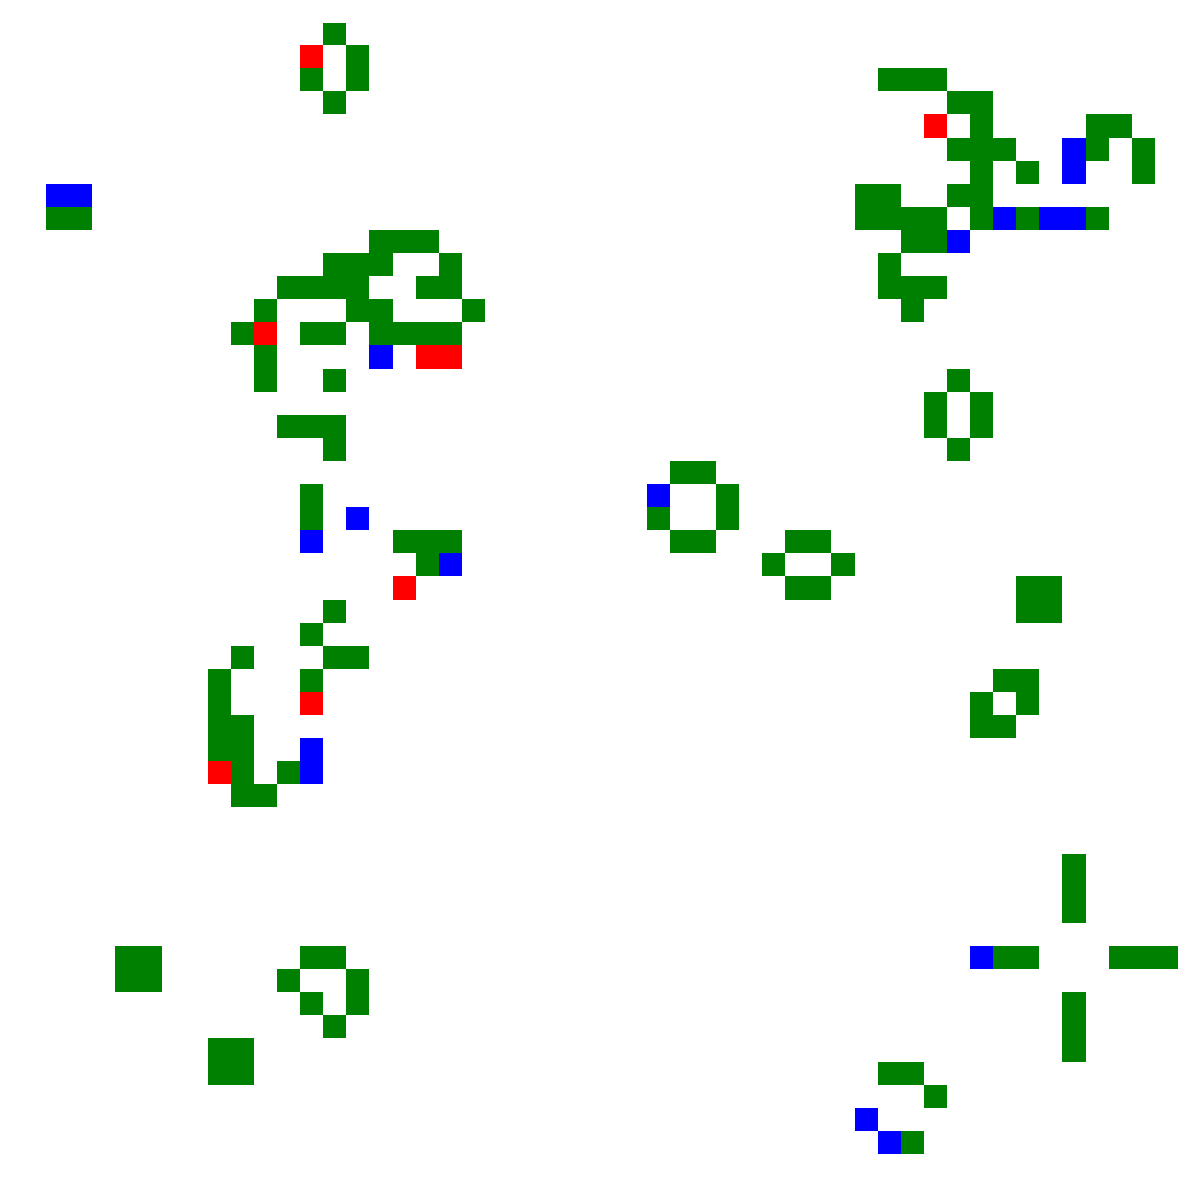
\includegraphics[width = 0.40\linewidth]{{../conway_plots/conway_static_p_0.5_pia_0.5_pii_0.3}.png}} \qquad
    \href{https://github.com/caam37830/project-group-8/blob/main/doc/final/conway_plots/conway_m_50_n_50_k_0.4_p_0.7_pia_0.6_pii_0.4.gif}{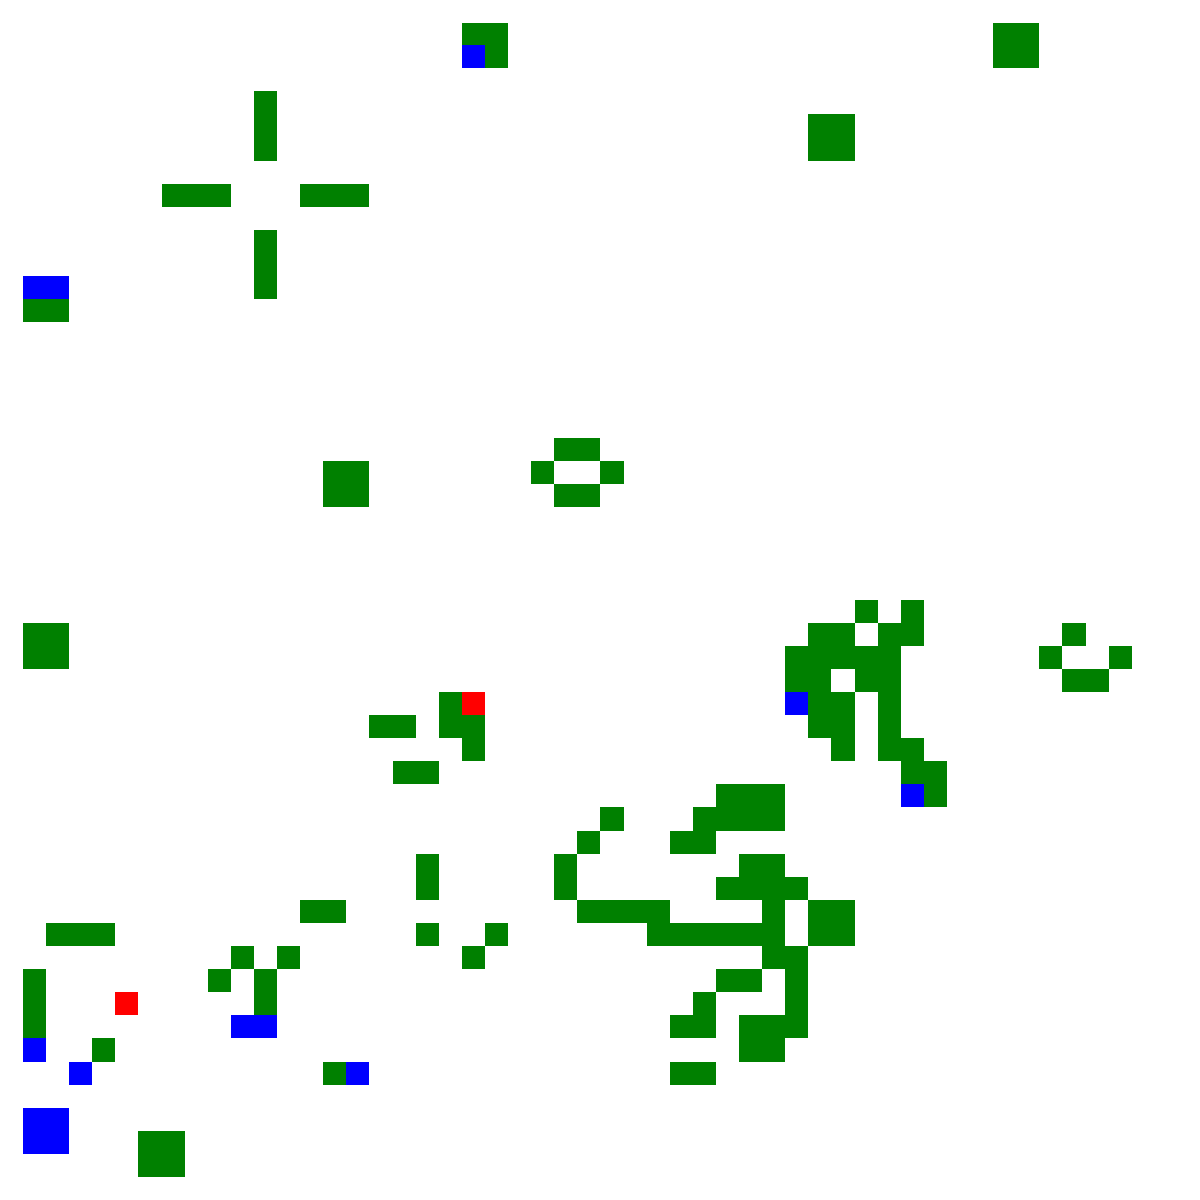
\includegraphics[width = 0.40\linewidth]{{../conway_plots/conway_static_p_0.7_pia_0.6_pii_0.4}.png}}
\end{center}
Some takeaways from watching \textbf{hours} of these animations (and the many hours of waiting for them to be compiled): first, the number of agents initially alive does not \emph{directly} affect the disease spread. When the proportion of initially alive agents is too high, many agents die from overcrowding before they are exposed to the disease, since Conway's game moves before the disease. Really, the number of agents which will be alive \emph{after} the first Conway ``move'' is what determines how many $t = 1$ infections there are.

Second, we see that green squares are sources of stability in the model; being ``recovered'' does not change the way Conway generates new grids, but it does allow some sort of herd-immunity effect: all four of these grids show red squares clinging on to green squares.

Third is that infection (at least empirically, from the footage I've seen) comes in ``waves'': because cells retain their state when they die, dead infected agents will be reborn as infected. If a square switches from dead to alive, after enough time periods, there is likely some sort of ``stable'' shape which flipped it to alive again (stable in the sense that there is a contiguous block of agents which will not all/mostly die on the next turn). This is similar to what we've seen in real life!


\section{Conclusions}
In the initial models, we observed that the discrete and continuous (ODE) versions of the model \emph{usually} ``agree'' in terms of output, but at certain critical values they can produce significantly different results, even in the long-run; this raises scientific and philosophical questions about which is a better model for real-world applications. When we introduced the spatial component, we found it to be a significant influence on the our discrete implementation, but rather insignificant in our ODE implementation.

From the smart agent extension, we derived a method of accounting for societal trends/behaviors in a discrete agent-based model. We empirically observed the effect of social distancing and the spread of social distancing trends, which serves as empirical motivation for future research on quantifying the effect of social distancing in real life.

From the reinfection extension, we derived a method of accounting for reinfection in an SIR model. We empirically observed a rebound in the proportion of the ``susceptible'' population, which stabilizes to a level roughly twice its minimum value over time. We also observe this curve ``compress'' and ``expand'' with respect to time as we change the rate of reinfect, $g$. Our findings motivate real-world research regarding the fluctuation in active cases for diseases which can be caught multiple times.

From the Conway Game of Life extension, we have not only invented a holiday wishlist \emph{must} for any fan of zero-player games, but also created a system which allows us to observe changes in the spread of the disease while incorporating movement: since Conway's Game is deterministic, which agents are ``alive'' at any time period will not change when re-running the model, only the random component -- the disease spread -- will. So Conway's Game of Life could be used to model different forms of movement (e.g. between homes, cities, countries), given suitable starting shapes of grids, knowledge of Conway's canonical \emph{pentominos}, and access to this Python package.


% -- Bibliography
\newpage{}                                    % Put the bibliography on a new page
\thispagestyle{empty}                         % Remove fancyhdr styling for the bibliography
\section*{Bibliography}                       % Make the bibliography an unnumbered section
\addcontentsline{toc}{section}{Bibliography}  % ...but make sure it's included in the table of contents
\begin{itemize}                               % List of references below
    \item Gardner, Martin.
        ``Mathematical Games -- The Fantastic Combinations of John Conway's New Solitaire Game 'Life' ''.
        Scientific American (223): 120–123, October 1970.
    \item Kamien, Morton I., and Nancy Lou Schwartz.
        ``Dynamic Optimization the Calculus of Variations and Optimal Control in Economics and Management''.
        Dover Publications, 2012.
    \item Murillo-Zamora E.; Mendoza-Cano O.; Delgado-Enciso I.; Hernandez-Suarez C. M.
        ``Predictors of Severe Symptomatic Laboratory-Confirmed Sars-Cov–2 Reinfection''.
        medRxiv 2020, 2020.10.14.20212720. 2020.
    \item Roos, Dave.
        ``Social Distancing and Quarantine Were Used in Medieval Times to Fight the Black Death.''
        History.com, A\&E Television Networks, \url{www.history.com/news/quarantine-black-death-medieval}.
        25 Mar. 2020.
    \item Wolfram, Stephen.
        ``A New Kind of Science''.
        Wolfram Media, Inc.
        p. 1179.
        ISBN 978-1-57955-008-0.
        2002.
\end{itemize}

\end{document}
